\documentclass[10pt, a4paper]{article}

% --- Packages ---
% \usepackage[margin=0.75in, top=1in]{geometry} % Adjust margins
% Tight margins for a datasheet look
\usepackage[left=0.75in, right=0.75in, top=0.5in, bottom=0.75in]{geometry}
\usepackage{graphicx}       % For the logo
\usepackage{xcolor}         % For colors
\usepackage{multicol}       % For two-column layout
\usepackage{titlesec}       % For custom section headers
\usepackage{enumitem}       % For list formatting
\usepackage{lmodern}       % Times New Roman-like font for body
\usepackage{helvet}         % Helvetica for headers
\usepackage{circuitikz}     % For the circuit diagram
\usepackage{tikz}           % For general drawing
\usepackage{booktabs}       % For nicer tables
\usepackage{multirow}       % For merging table cells
\usepackage{tabularx}       % For flexible tables
\usepackage{amsmath}        % For math symbols like \pm


% --- Custom Colors ---
% Approximating the "Analog Devices" red/maroon
\definecolor{headerred}{RGB}{160, 20, 30}

% --- Font & Section Setup ---
% Define a custom font command for the big headers
\newcommand{\datasheetheader}[1]{%
    {\fontfamily{phv}\selectfont\bfseries\color{headerred}\LARGE\MakeUppercase{#1}}%
}

% Customize standard \section to look like the datasheet headers
\titleformat{\section}
  {\fontfamily{phv}\selectfont\bfseries\color{headerred}\Large\MakeUppercase} % Format
  {} % Label
  {0pt} % Sep
  {} % Before code

\titlespacing*{\section}{0pt}{10pt}{5pt}
% This defines "C" as a Centered version of the "X" column
\newcolumntype{C}{>{\centering\arraybackslash}X}
% Remove paragraph indentation
\setlength{\parindent}{0pt}

%
% --- Header & Footer Setup ---
\usepackage{fancyhdr}
\pagestyle{fancy} % Turn on the fancy style
\fancyhf{} % Clear all default headers and footers

% 1. Define the thick colored Header Line
\renewcommand{\headrule}{%
    {\color{headerred}\hrule height 2pt}%
    \vspace{2pt} % Add a little space between line and body text
}

% 2. Define the thick colored Footer Line
\renewcommand{\footrule}{%
    \vspace{2pt} % Add a little space between body text and line
    {\color{headerred}\hrule height 2pt}%
}

% 3. Set the text content (Optional)
\fancyhead[L]{\small \textbf{R\&T BiCMOS}}    % Top Left
\fancyhead[R]{\small \textbf{B.TON - APC}} % Top Right
\fancyfoot[C]{\thepage}                   % Bottom Center (Page Number)

% --- Fix for head height warning ---
% Because the line is 7pt thick, you might need to increase headheight
\setlength{\headheight}{25pt}
%

\begin{document}

% ==========================================
% HEADER SECTION
% ==========================================
\begin{minipage}[b]{0.4\textwidth}
    % Placeholder for Logo. Replace example-image with your logo file.
    \includegraphics[width=1.5cm]{image/logo/RetT_black.PNG} \\
    {\fontfamily{phv}\selectfont\bfseries\Huge\hspace{3pt} \scalebox{1.0}{R\&T BiCMOS}}
\end{minipage}%
\hfill
\begin{minipage}[b]{0.55\textwidth}
    \raggedleft
    % {\fontfamily{phv}\selectfont\Huge\bfseries Run2}\\[5pt]
    {\fontfamily{phv}\selectfont\Huge Low Noise, Cryogenic \\ Differential Amplifier}
\end{minipage}

\vspace{5pt}
{\color{headerred}\hrule height 7pt}
\vspace{10pt}
Prepared by: Bao TON

% ==========================================
% TWO-COLUMN BODY
% ==========================================
\begin{multicols}{2}

    % --- DESCRIPTION ---
    \section*{Description}
    The RH6200 is an ultralow noise, rail-to-rail input and output unity-gain stable op amp that features $0.95\text{nV}/\sqrt{\text{Hz}}$ noise voltage. This amplifier combines very low noise with a 165MHz gain bandwidth, 50V/$\mu$s slew rate and is optimized for low voltage signal conditioning systems. A shutdown pin reduces supply current during standby conditions and thermal shutdown protects the part from overload conditions. The RH6200 maintains its pre-irradiation performance for supplies from 4.5V to 12.6V and is specified pre- and post-radiation at 5V and $\pm$5V.

    % --- ABSOLUTE MAXIMUM RATINGS ---
    \section*{Absolute Maximum Ratings}
    \textbf{(Note 1)}
    
    \begin{tabbing}
        \hspace{6cm} \= \kill
        Total Supply Voltage ($\text{V}^+$ to $\text{V}^-$) \> 12.6V \\
        \dotfill \\
        Input Current (Note 2) \> $\pm$40mA \\
        \dotfill \\
        Output Short-Circuit Duration (Note 3) \> Indefinite \\
        \dotfill \\
        Pin Current While Exceeding Supplies (Note 4) \> $\pm$30mA \\
        \dotfill \\
        Operating Junction Temperature Range \\
        \hspace{0.5cm} (Note 5) \> $-55^\circ$C to $125^\circ$C \\
        \dotfill \\
        Storage Temperature Range \> $-65^\circ$C to $150^\circ$C \\
        \dotfill \\
        Lead Temperature (Soldering, 10 sec) \> $300^\circ$C \\
    \end{tabbing}
    {\tiny All registered trademarks and trademarks are the property of their respective owners.}

\end{multicols}

\vspace{5pt}
{\color{headerred}\hrule height 2pt}
\vspace{10pt}

\begin{multicols}{2}

    % --- BURN-IN CIRCUIT ---
    \section*{Burn-In Circuit}
    \vspace{0.5cm}
    \begin{center}
    \begin{circuitikz}[scale=0.8, transform shape]
        % Opamp
        \draw (2,2) node[op amp] (opamp) {};
        
        % Resistors and inputs
        \draw (opamp.-) -- ++(-0.5,0) coordinate(neg_in);
        \draw (neg_in) -- ++(0, 1.5) to[R, l=10k, name=R1] ++(2.5,0) -| (opamp.out);
        \draw (neg_in) to[R, l=200$\Omega$] ++(-1.5,0) node[ground] {};
        
        \draw (opamp.+) -- ++(-0.5,0) to[R, l=10k] ++(-1.5,0) node[ground] {};
        
        % Power rails
        \draw (opamp.up) -- ++(0,0.5) node[above] {6.3V};
        \draw (opamp.down) -- ++(0,-0.5) node[below] {-6.3V};
        
        % Pin Numbers (Manual placement)
        \node[font=\tiny] at (opamp.bin 1) [above left] {3};
        \node[font=\tiny] at (opamp.bin 2) [below left] {4};
        \node[font=\tiny] at (opamp.bout) [above right] {7};
        \node[font=\tiny] at (opamp.up) [right] {8};
        \node[font=\tiny] at (opamp.down) [right] {5};
        
        \node[font=\tiny] at (2,-1.5) {RH6200M F01};
    \end{circuitikz}
    \end{center}

    % --- PACKAGE INFO ---
    \section*{Package/Order Information}
    
    \begin{tabular}{|c|c|}
        \hline
        \begin{tabular}{c}
             \textbf{ORDER PART} \\
             \textbf{NUMBER} \\
             \hline
             RH6200MW \\
        \end{tabular} 
        & 
        \begin{minipage}{0.25\textwidth}
            \centering
            \tiny TOP VIEW
            \vspace{5pt}
            \begin{tikzpicture}[scale=0.6]
                % Chip Body
                \draw[thick] (0,0) rectangle (2,2.5);
                % Pins Left
                \foreach \y/\lab in {2.2/SHDN 1, 1.8/NC 2, 1.4/-IN 3, 1.0/+IN 4, 0.6/V$^-$ 5} {
                    \draw (0,\y) -- (-0.3,\y); 
                    \draw (-0.3,\y-0.1) rectangle (0,\y+0.1);
                    \node[anchor=east, font=\tiny] at (-0.3,\y) {\lab};
                }
                % Pins Right
                \foreach \y/\lab in {2.2/10 NC, 1.8/9 NC, 1.4/8 V$^+$, 1.0/7 OUT, 0.6/6 NC} {
                    \draw (2,\y) -- (2.3,\y);
                    \draw (2,\y-0.1) rectangle (2.3,\y+0.1);
                    \node[anchor=west, font=\tiny] at (2.3,\y) {\lab};
                }
                % Triangle inside
                \draw (0.5, 0.8) -- (0.5, 1.8) -- (1.5, 1.3) -- cycle;
                \node at (0.7, 1.1) {\tiny +};
                \node at (0.7, 1.5) {\tiny -};
            \end{tikzpicture}
            \\
            \tiny W PACKAGE\\
            \tiny 10-LEAD CERPAC
        \end{minipage}
        \\ \hline
    \end{tabular}

\end{multicols}
\vspace{5pt}
{\color{headerred}\hrule height 2pt}
\vspace{10pt}
\section*{TABLE 1: ELECTRICAL CHARACTERISTICS}
\renewcommand{\arraystretch}{1.2}
\begin{table}[ht]
    \centering
    % Resizebox ensures the table fits the page regardless of column widths
    \resizebox{\textwidth}{!}{%
    
        % Note: I changed 'C' to 'm{3.5cm}' in the line below
        \begin{tabularx}{1.55\textwidth}{l|l|m{3.5cm}|c|ccc|c|ccc|c|c}
            \hline
            \multirow{2}{*}{\textbf{SYMBOL}} & 
            \multirow{2}{*}{\textbf{PARAMETER}} & 
            \multirow{2}{*}{\centering \textbf{CONDITIONS}} & % Added \centering here manually
            \multirow{2}{*}{\textbf{NOTES}} & 
            \multicolumn{3}{c|}{$\mathbf{T_A = 25^\circ C}$} & 
            \multirow{2}{*}{\parbox{1.5cm}{\centering \textbf{SUB-}\\ \textbf{GROUP}}} & 
            \multicolumn{3}{c|}{$\mathbf{-55^\circ C \le T_A \le 125^\circ C}$} & 
            \multirow{2}{*}{\parbox{1.5cm}{\centering \textbf{SUB-}\\ \textbf{GROUP}}} & 
            \multirow{2}{*}{\textbf{UNITS}} \\
            
            \cline{5-7} \cline{9-11}
             & & & & \textbf{MIN} & \textbf{TYP} & \textbf{MAX} & & \textbf{MIN} & \textbf{TYP} & \textbf{MAX} & & \\
            \hline
            
            $V_{OS}$ & Input Offset & \centering $V_S = 5\text{V}, 0\text{V};$ & & & 0.6 & 2 & 1 & & & 4 & 2,3 & mV \\
                     & Voltage      & \centering $V_{CM} = V^-\text{ to }V^+$ & & & 2.5 & 6 & 1 & & & 9 & 2,3 & mV \\
            \hline
            $I_B$    & Input Bias   & \centering $V_S = 5\text{V}, 0\text{V};$ & & & 8 & 18 & 1 & & & 20 & 2,3 & $\mu$A \\
                     & Current      & \centering $V_{CM} = V^+$               & & -50 & -23 & & 1 & -100 & & & 2,3 & $\mu$A \\
            \hline
        \end{tabularx}%
    }
\end{table}
\end{document}